% !TEX program = xelatex
% 第二讲：stationary.tex + classification.tex
\documentclass[fontset=windows, chinese, 10pt, xcolor=dvipsnames]{beamer}
% Shared preamble for the chapter 05 standalone lectures.
% Each lecture sets \title and \subtitle after this file is read.

\usepackage{amsmath,amssymb,mathtools}
\usepackage{xeCJK}
\usepackage{zhnumber}
\usepackage{tikz}
\usetikzlibrary{arrows.meta,calc,positioning}

\usetheme{metropolis}
\usepackage{beamercolorthemeHistNanjing}

\newcommand{\red}[1]{\textcolor{red}{#1}}
\newcommand{\blue}[1]{\textcolor{blue}{#1}}
\newcommand{\green}[1]{\textcolor{green}{#1}}
\newcommand{\gray}[1]{\textcolor{gray}{#1}}
\newcommand{\orange}[1]{\textcolor{orange}{#1}}

\newcommand{\sssub}[1]{ {\mathrm{#1} }}  % script size subscript\\\
\newcommand{\funcd}[2]{ \frac{d{#1}}{d{#2}}} %function full derivative
\newcommand{\funcpd}[2]{ \frac{\partial{#1}}{\partial{#2}}} %function partial derivative
\newcommand{\fnald}[2] { \frac{\delta {#1}}{\delta {#2}}} % functional derivative

\renewcommand{\Re}{\operatorname{Re}}
\renewcommand{\Im}{\operatorname{Im}}
\def\ext{\sssub{ext}}
\def\x{\sssub{x}}
\def\xc{\sssub{xc}}
\def\H{\sssub{H}}
\def\Hx{\sssub{Hx}}
\def\Hxc{\sssub{Hxc}}
\def\c{\sssub{c}}
\def\s{\sssub{s}}

% \def\ext{\sssub{ext}}
% \def\ext{\sssub{ext}}
% \def\ext{\sssub{ext}}
% \def\ext{\sssub{ext}}
% \defsssub{ext}


% definitions of bold faced symbols
\def\brpppp{{\mathbf{r}^{\prime\prime\prime\prime}}}
\def\brppp{{\mathbf{r}^{\prime\prime\prime}}}
\def\brpp{{\mathbf{r}^{\prime\prime}}}
\def\brp{{\mathbf{r}^{\prime}}}
\def\bzp{{\mathbf{z}^{\prime}}}
\def\bxp{{\mathbf{x}^{\prime}}}
\def\tp{{{t}^{\prime}}}
\def\tpp{{{t}^{\prime\prime}}}
\def\tppp{{{t}^{\prime\prime\prime}}}

\def\tbr{{\tilde{\mathbf{r}}}}
\def\bk{{\mathbf{k}}}
\def\br{{\mathbf{r}}}
\def\bp{{\mathbf{p}}}
\def\bq{{\mathbf{q}}}
\def\bv{{\mathbf{v}}}
\def\bz{{\mathbf{z}}}
\def\mbf{{\mathbf{f}}}

\def\bx{{\mathbf{x}}}
\def\bR{{\mathbf{R}}}
\def\bM{{\mathbf{M}}}
\def\bP{{\mathbf{P}}}
\def\bT{{\mathbf{T}}}
\def\bK{{\mathbf{K}}}
\def\bA{{\mathbf{A}}}
\def\bB{{\mathbf{B}}}
\def\bD{{\mathbf{D}}}
\def\bE{{\mathbf{E}}}
\def\bF{{\mathbf{F}}}
\def\bG{{\mathbf{G}}}
\def\bH{{\mathbf{H}}}
\def\bI{{\mathbf{I}}}
\def\bJ{{\mathbf{J}}}
\def\bP{{\mathbf{P}}}
\def\bS{{\mathbf{S}}}
\def\bV{{\mathbf{V}}}
\def\bX{{\mathbf{X}}}
\def\bY{{\mathbf{Y}}}
\def\dd{{\mathop{}\!\mathrm{d}}}
\def\dr{{\!\!\dd\br\,}}
\def\dx{{\!\!\dd\bx\,}}
\def\dy{{\!\!\dd\by\,}}
\def\dk{{\!\!\dd\bk\,}}
\def\dG{{\!\!\dd\bG\,}}


\def\half{{\frac{1}{2}}}
\def\tr{{\mathrm{tr}}}


\def\Arg{{\mathrm{Arg}\;}}
\def\arg{{\mathrm{arg}\;}}
\def\Res{{\mathrm{Res}\;}}


\author{罗凯}
\institute{南京理工大学物理学院}
\date{\zhdigits{\the\year},\zhganzhinian{\the\year}年秋}

\usebackgroundtemplate{%
\begin{tikzpicture}[remember picture,overlay]
  \node[opacity=0.05, at=(current page.center)] {
    
\includegraphics[width=0.6\paperwidth]{njust-logo.jpeg}
  };
\end{tikzpicture}}


\title{数学物理方程}
\subtitle{第二讲：定解条件与方程分类}

\begin{document}

\begin{frame}
  \titlepage
\end{frame}

\begin{frame}{承接上一讲}
  上一讲得到了三条标准方程：
  \begin{align*}
    u_{tt}-a^2u_{xx}&=f,\\
    u_t&=\kappa\nabla^2u+f,\\
    \nabla^2u&=f.
  \end{align*}
  它们表达的是局部物理规律。本讲回答：哪一个函数才是眼前这个系统的解，以及这三类方程为什么行为不同。
\end{frame}

\begin{frame}{本讲提纲}
  \begin{enumerate}
    \item 用同一个波动方程的三个解，说明为什么还要初始数据；
    \item 先看弦的三种端点，再写成狄利克雷、诺伊曼、罗宾条件；
    \item 用两个模态看叠加，再做一块平板的稳态导热；
    \item 先对三个方程算判别式，再讲特征线和标准形。
  \end{enumerate}
\end{frame}

% =============================================================
\section{定解条件}

\subsection{从方程到定解问题}

\begin{frame}{方程不是一个完整的物理情形}
  偏微分方程的\textbf{解}，是足够光滑、具有方程所要求的全部导数，并且在区域内使方程成为恒等式的函数。
  \vspace{0.4em}

  只找到方程，只完成了物理问题的前一半。方程单独通常有无穷多个解。要选出实际系统对应的那一个，还需要描述初始状态以及系统与边界如何作用的数据。
  \vspace{0.4em}

  方程加上这些补充数据，称为\textbf{初边值问题}（initial-boundary-value problem）。
\end{frame}

\begin{frame}{同一个方程的三种运动}
  下面三个函数都满足 $u_{tt}-a^2u_{xx}=0$，并且 $u(0,t)=u(\ell,t)=0$：
  \begin{align*}
    u_0&=0,\\
    u_1&=\sin\Bigl(\frac{\pi x}{\ell}\Bigr)
        \cos\Bigl(\frac{\pi a t}{\ell}\Bigr),\\
    u_2&=\sin\Bigl(\frac{2\pi x}{\ell}\Bigr)
        \cos\Bigl(\frac{2\pi a t}{\ell}\Bigr).
  \end{align*}
  $u_1$ 是从静止松开的半个正弦；$u_2$ 中间有一个不动的节点。方程和固定端留住了这三种运动，初始形状才把它们分开。
\end{frame}

\begin{frame}{两端固定的弦}
  波动方程 $u_{tt}-a^2u_{xx}=0$ 要配上
  \begin{equation*}
    u(0,t)=u(\ell,t)=0,
    \qquad
    u(x,0)=\varphi(x),\quad u_t(x,0)=\psi(x).
  \end{equation*}
  \begin{itemize}
    \item $\varphi$ 是初始位移，$\psi$ 是初始速度。它们从波动方程的许多解里选出一种运动。
    \item 端点条件表示支座不动。
  \end{itemize}
  二阶时间方程需要两个初始数据，和牛顿定律需要位置与速度是同一件事。
\end{frame}

\begin{frame}{完整的定解问题}
  若还有力密度 $f(x,t)$，两端固定的弦可以写成
  \begin{equation*}
    \left\{
    \begin{aligned}
      u_{tt}-a^2u_{xx}&=f(x,t),
        && 0<x<\ell,\ t>0,\\
      u(x,0)&=\varphi(x),\quad u_t(x,0)=\psi(x),
        && 0\leq x\leq\ell,\\
      u(0,t)&=0,\quad u(\ell,t)=0,
        && t\geq 0.
    \end{aligned}
    \right.
  \end{equation*}
  方程描述任何小弦振动都遵守的规律；初始数据和边界数据指定眼前这一次振动。
\end{frame}

\begin{frame}{数据写在时空区域的什么地方}
  \begin{columns}[c]
    \begin{column}{0.48\textwidth}
      \begin{itemize}
        \item 开带形 $0<x<\ell$、$t>0$ 内满足方程。
        \item $t=0$ 这段上给出初始位移和初始速度。
        \item 两条竖直线 $x=0$、$x=\ell$ 上给出端点数据。
      \end{itemize}
      解在闭区域上连续时，角点上的初始数据和边界数据必须一致，例如 $\varphi(0)=\varphi(\ell)=0$。
    \end{column}
    \begin{column}{0.48\textwidth}
      \centering
      \begin{tikzpicture}[scale=0.78]
        \draw[->] (0,0) -- (4.3,0) node[right] {$x$};
        \draw[->] (0,0) -- (0,3.3) node[above] {$t$};
        \draw[thick,red] (0,0) -- (3.3,0);
        \draw[thick,blue] (0,0) -- (0,2.8);
        \draw[thick,blue] (3.3,0) -- (3.3,2.8);
        \node[below] at (0,0) {$0$};
        \node[below] at (3.3,0) {$\ell$};
        \node[red,below] at (1.65,-0.55) {$\varphi,\psi$};
        \node[blue,left] at (0,1.6) {$u=0$};
        \node[blue,right] at (3.3,1.6) {$u=0$};
        \node at (1.65,1.5) {方程};
      \end{tikzpicture}
    \end{column}
  \end{columns}
\end{frame}

\subsection{三类边界条件}

\begin{frame}{先看弦的三种端点}
  边界条件先从端点上的力看，再起名字。
  \begin{itemize}
    \item 端点钉死：$u(0,t)=0$。指定的是位移本身。
    \item 端点自由：横向力为零，小斜率下就是 $u_x(0,t)=0$。指定的是斜率。
    \item 端点连着弹簧：张力的横向分量与弹簧拉力平衡，位移和斜率一起出现。
  \end{itemize}
  温度和电势也是这三种问法：边界上的值、穿过边界的通量，或二者的一个组合。
\end{frame}

\begin{frame}{狄利克雷条件}
  狄利克雷条件把场在边界上的值规定死。
  \begin{itemize}
    \item 弦拴在不动的支座上：$u(0,t)=u(\ell,t)=0$，或更一般地等于给定的端点运动。
    \item 物体表面保持在指定温度。
    \item 导体表面是等势面，电势可取为给定常数。
  \end{itemize}
  指定的是未知函数本身，不是它的导数。
\end{frame}

\begin{frame}{诺伊曼条件}
  对弦，$u_x(0,t)=0$ 表示自由端：张力的横向分量为零，端点在横向上不受力。
  \vspace{0.3em}

  更一般地，
  \begin{equation*}
    u_x(0,t)=\mu(t)
  \end{equation*}
  给出端点上随时间变化的横向力。这是第二类，也就是诺伊曼边界条件。
  \vspace{0.3em}

  在热传导里，法向导数对应热通量。绝热边界就是法向通量为零。
\end{frame}

\begin{frame}{罗宾条件}
  第三类边界条件可以描述弹性支承。设弹簧常数为 $k$，端点位移就是弹簧的伸长。在 $x=\ell$ 处力平衡给出
  \begin{equation*}
    T u_x(\ell,t)+k u(\ell,t)=0,
  \end{equation*}
  也就是 $u_x+\sigma u=0$，$\sigma=k/T$。
  \vspace{0.4em}

  更一般的形式 $u_x+\sigma u=v(t)$ 同时包含外加的端点力和弹性恢复力。热传导中的牛顿冷却定律也是这一类：热通量与表面和环境的温差成正比。
\end{frame}

\begin{frame}{抽象成三类}
  在一般空间区域 $\Omega$ 上，刚才三种端点写成
  \begin{align*}
    u\big|_{\partial\Omega}&=g
      && \text{狄利克雷：指定场本身},\\
    \frac{\partial u}{\partial n}\bigg|_{\partial\Omega}&=h
      && \text{诺伊曼：指定法向通量或斜率},\\
    \alpha u+\beta\frac{\partial u}{\partial n}&=r
      && \text{罗宾：场和通量耦合在一起}.
  \end{align*}
  它们也依次称为第一、第二、第三类边界条件。名字不同，问的都是：边界上已知的是值、通量，还是二者的关系。
\end{frame}

% =============================================================
\section{线性结构与叠加}

\subsection{阶、线性与非线性}

\begin{frame}{阶与线性}
  方程的\textbf{阶}是最高阶导数的阶。弦振动方程是二阶的。
  \vspace{0.4em}

  若 $u$ 和它的所有导数都线性出现，而且系数不依赖于 $u$，方程就是\textbf{线性}的。否则是非线性的。
  \vspace{0.4em}

  上一讲的波动、热传导、拉普拉斯和泊松方程，在系数给定时都是线性的。纳维--斯托克斯方程和伯格斯方程不是。
\end{frame}

\begin{frame}{拟线性与完全非线性}
  非线性方程如果最高阶导数仍然线性出现，就称为\textbf{拟线性}。例如
  \begin{equation*}
    u_t+u u_x=0
  \end{equation*}
  是一阶拟线性的：$u_t$ 和 $u_x$ 的系数不依赖导数，但 $u_x$ 的系数依赖 $u$。
  \vspace{0.4em}

  相反，
  \begin{equation*}
    u_x^2+u_y^2=u
  \end{equation*}
  是完全非线性的，因为最高阶导数不以线性方式出现。分类理论下面只对线性二阶方程展开。
\end{frame}

\begin{frame}{齐次与非齐次}
  含有非零已知源，例如定解问题里的 $f(x,t)$，方程就是\textbf{非齐次}的；去掉源之后的方程是\textbf{齐次}的。
  \vspace{0.4em}

  边界条件同样区分：
  \begin{itemize}
    \item $u(0,t)=u(\ell,t)=0$ 是齐次边界条件；
    \item 端点位移被规定成非零函数时，边界条件是非齐次的。
  \end{itemize}
  初始条件只有在 $\varphi$ 和 $\psi$ 都为零时才是齐次的。
\end{frame}

\begin{frame}{例：两个纯音可以相加}
  取前面的
  \begin{equation*}
    u_1=\sin\Bigl(\frac{\pi x}{\ell}\Bigr)\cos\Bigl(\frac{\pi at}{\ell}\Bigr),
    \quad
    u_2=\sin\Bigl(\frac{2\pi x}{\ell}\Bigr)\cos\Bigl(\frac{2\pi at}{\ell}\Bigr).
  \end{equation*}
  $u_1+u_2$ 和 $3u_1$ 仍满足波动方程与固定端：每一项已经满足，导数又是线性的。
  \vspace{0.3em}

  $u_1+x$ 则不行。$x$ 自己不满足波动方程，端点也不再是零。能叠加的是\textbf{同一个齐次问题}的解，不是任意函数。
\end{frame}

\begin{frame}{叠加原理}
  齐次线性问题特别重要，因为有叠加原理：若 $u_1,u_2$ 满足同一个齐次线性方程和同一组齐次边界条件，则
  \begin{equation*}
    c_1u_1+c_2u_2
  \end{equation*}
  也满足。
  \vspace{0.4em}

  分离变量法利用的就是这件事：先找一批乘积形式的特解，再把它们加起来配合初始数据。非齐次项或非齐次边界条件破坏直接叠加，要先作展开或把边界条件齐次化。第三讲处理弦上的外力时会看到前一种做法。
\end{frame}

\begin{frame}{演化问题与稳态问题}
  平衡问题没有初始时刻的演化。人们在空间边界上指定数据，去解椭圆型边值问题，例如 $\nabla^2u=0$ 或 $\nabla^2u=f$。
  \vspace{0.4em}

  物理上，稳态解是源、通量和约束已经平衡、可观测的场不再随时间改变的状态。
  \begin{itemize}
    \item 初始条件自然属于演化方程。
    \item 边界条件对演化问题和稳态问题都必不可少。
  \end{itemize}
\end{frame}

% =============================================================
\section{稳态问题}

\subsection{解题步骤}

\begin{frame}{稳态问题在问什么}
  演化问题问：从给定的初始状态出发，状态怎样变化。
  \vspace{0.3em}

  稳态问题问：哪一个不随时间变化的场，能同时配合源和边界数据。
  \vspace{0.3em}

  把演化方程里的每一个时间导数设为零，就是从前者走到后者的第一步。下面用一块平板把整条路线走完，再把步骤收成清单。
\end{frame}

\begin{frame}{例：无源平板的稳态导热}
  均匀平板 $0\leq x\leq L$，传导系数 $k$ 为常数，内部无热源，边界温度为
  \begin{equation*}
    u(0)=T_0,\qquad u(L)=T_L.
  \end{equation*}
  含时方程是 $u_t=\kappa u_{xx}$。第一步令 $u_t=0$，得到
  \begin{equation*}
    u''(x)=0.
  \end{equation*}
  这是一维拉普拉斯方程。积分两次，
  \begin{equation*}
    u(x)=Ax+B.
  \end{equation*}
\end{frame}

\begin{frame}{例：用两端温度定常数}
  $x=0$ 给出 $B=T_0$。$x=L$ 给出 $A=(T_L-T_0)/L$。因此
  \begin{equation*}
    \boxed{u(x)=T_0+\frac{T_L-T_0}{L}x.}
  \end{equation*}
  内部没有源，温度才是线性的。热通量
  \begin{equation*}
    q_x=-k\frac{\mathrm{d}u}{\mathrm{d}x}
    =-k\frac{T_L-T_0}{L}
  \end{equation*}
  为常数：每一薄片流入和流出的热量相等，这正是稳态平衡。
\end{frame}

\begin{frame}{有源时只改方程那一步}
  内部有源时，变的是求解微分方程的那一步，步骤本身不变。均匀源 $F$ 给出 $u''=-F/k$，稳态剖面是抛物线
  \begin{equation*}
    u(x)=\frac{F}{2k}x(L-x)
  \end{equation*}
  （两端温度为零时）。这就是上一讲的加热板。
  \vspace{0.4em}

  多维时变难的是选择坐标和确定系数：矩形用直角坐标，圆和球用极坐标或球坐标。第三讲做两个完整的例子。
\end{frame}

\begin{frame}{刚才的平板，收成六步}
  \begin{enumerate}
    \item 确认未知场，令演化方程中所有时间导数为零。平板上令 $u_t=0$。
    \item 写明区域，把边界翻译成狄利克雷、诺伊曼或罗宾条件。这里是 $u(0)=T_0$，$u(L)=T_L$。
    \item 判断有没有源。无源得到 $u''=0$，有均匀源得到 $u''=-F/k$。
    \item 按几何选择坐标。这块平板只用 $x$。
    \item 用边界条件定常数。$B=T_0$，$A=(T_L-T_0)/L$。
    \item 代回去检查。通量 $q_x$ 为常数，流入等于流出；若 $T_L=T_0$，则 $u$ 是常数，通量为零。
  \end{enumerate}
\end{frame}

% =============================================================
\section{方程分类}

\subsection{一般二阶线性方程}

\begin{frame}{为什么要分类}
  上一讲的三个方程，解的行为明显不同：波动把信号以有限速度送出去，热传导把差异抹平，拉普拉斯方程描述平衡。
  \vspace{0.4em}

  差别编码在最高阶导数那一部分，也就是方程的\textbf{主部}。低阶项可以改变衰减和源，但不决定类型。
  \vspace{0.4em}

  顺序是：先写出判别式，并对波动、热传导、拉普拉斯三个方程各算一次；再说明特征线；最后用换元证明类型与坐标无关，并化成标准形。
\end{frame}

\begin{frame}{两个自变量}
  两个自变量的线性二阶方程写成
  \begin{equation*}
    A u_{xx}+2B u_{xy}+C u_{yy}
    +D u_x+E u_y+Fu=G.
  \end{equation*}
  系数 $A,B,C,D,E,F,G$ 是 $x,y$ 的已知实函数。这里的 $x,y$ 是一对自变量的名字：可以都是空间坐标，也可以一个是时间。
  \vspace{0.3em}

  方程和数据都是线性的，所以方程与数据分别叠加时，解也叠加。
\end{frame}

\begin{frame}{多个自变量}
  对自变量 $x_1,\ldots,x_n$，二阶线性方程是
  \begin{equation*}
    \sum_{i,j=1}^n a_{ij}(\mathbf{x})\,u_{x_ix_j}
    +\sum_{i=1}^n b_i(\mathbf{x})\,u_{x_i}
    +c(\mathbf{x})\,u+f(\mathbf{x})=0.
  \end{equation*}
  两个自变量时，分类和化成标准形都可以直接写出来。下面只做这一情形。
\end{frame}

\begin{frame}{判别式}
  对 $A u_{xx}+2B u_{xy}+C u_{yy}+\cdots=0$，定义
  \begin{equation*}
    \Delta=B^2-AC.
  \end{equation*}
  在主部系数不同时为零的点，
  \begin{center}
  \begin{tabular}{lll}
    $\Delta>0$ & 双曲型 & 波动式传播\\
    $\Delta=0$ & 抛物型 & 扩散式演化\\
    $\Delta<0$ & 椭圆型 & 平衡或势场
  \end{tabular}
  \end{center}
  \vspace{0.4em}
  系数变化时，类型可以随区域改变。判断类型不用先换坐标。
\end{frame}

\begin{frame}{三个标准例子的判别式}
  写明哪个变量充当一般形式里的 $x,y$。
  \begin{itemize}
    \item 波动 $u_{tt}-a^2u_{xx}=0$：第一变量取 $t$，则 $A=1$，$B=0$，$C=-a^2$，$\Delta=a^2>0$，双曲。
    \item 热传导 $u_t-\kappa u_{xx}=0$：没有 $u_{tt}$。若第一变量取 $x$，则 $A=-\kappa$，$B=C=0$，$\Delta=0$，抛物。
    \item 拉普拉斯 $u_{xx}+u_{yy}=0$：$A=C=1$，$B=0$，$\Delta=-1<0$，椭圆。
  \end{itemize}
  上一讲的三个行为——振荡传播、抹平、平衡——正好是这三种符号。
\end{frame}

\subsection{换元与特征线}

\begin{frame}{非奇异的自变量替换}
  作非奇异变换
  \begin{equation*}
    \xi=\xi(x,y),\qquad \eta=\eta(x,y),
    \qquad
    \frac{\partial(\xi,\eta)}{\partial(x,y)}\neq 0.
  \end{equation*}
  链式法则先给出
  \begin{align*}
    u_x&=u_\xi\xi_x+u_\eta\eta_x,\\
    u_y&=u_\xi\xi_y+u_\eta\eta_y.
  \end{align*}
  雅可比不为零，保证新坐标在局部真的是一组坐标，类型不会被退化的换元弄假。
\end{frame}

\begin{frame}{二阶导数}
  再求一次导数：
  \begin{align*}
    u_{xx}={}&u_{\xi\xi}\xi_x^2+2u_{\xi\eta}\xi_x\eta_x
      +u_{\eta\eta}\eta_x^2
      +u_\xi\xi_{xx}+u_\eta\eta_{xx},\\[4pt]
    u_{yy}={}&u_{\xi\xi}\xi_y^2+2u_{\xi\eta}\xi_y\eta_y
      +u_{\eta\eta}\eta_y^2
      +u_\xi\xi_{yy}+u_\eta\eta_{yy}.
  \end{align*}
  $u_{xy}$ 同样展开后含有 $u_{\xi\xi}$、$u_{\xi\eta}$、$u_{\eta\eta}$，以及 $u_\xi,u_\eta$ 乘坐标二阶导数的低阶项。
\end{frame}

\begin{frame}{混合导数与变换后的方程}
  \begin{align*}
    u_{xy}={}&u_{\xi\xi}\xi_x\xi_y
      +u_{\xi\eta}(\xi_x\eta_y+\xi_y\eta_x)
      +u_{\eta\eta}\eta_x\eta_y\\
      &+u_\xi\xi_{xy}+u_\eta\eta_{xy}.
  \end{align*}
  代入原方程后仍是线性的：
  \begin{equation*}
    A_{11}u_{\xi\xi}+2A_{12}u_{\xi\eta}+A_{22}u_{\eta\eta}
    +B_1u_\xi+B_2u_\eta+\widetilde C u+\widetilde F=0.
  \end{equation*}
\end{frame}

\begin{frame}{新的主部系数}
  \begin{align*}
    A_{11}&=A\xi_x^2+2B\xi_x\xi_y+C\xi_y^2,\\
    A_{12}&=A\xi_x\eta_x+B(\xi_x\eta_y+\xi_y\eta_x)+C\xi_y\eta_y,\\
    A_{22}&=A\eta_x^2+2B\eta_x\eta_y+C\eta_y^2.
  \end{align*}
  主部系数是旧系数 $(A,B,C)$ 的二次型，作用在新坐标的梯度上。分类只看它们。
\end{frame}

\begin{frame}{低阶系数}
  化成完整的新方程时还需要
  \begin{align*}
    B_1&=A\xi_{xx}+2B\xi_{xy}+C\xi_{yy}+D\xi_x+E\xi_y,\\
    B_2&=A\eta_{xx}+2B\eta_{xy}+C\eta_{yy}+D\eta_x+E\eta_y,\\
    \widetilde C&=F,\qquad \widetilde F=-G.
  \end{align*}
  这些项不影响类型。坐标二阶导数出现在 $B_1,B_2$ 里，是因为链式法则作用在一阶导数上。
\end{frame}

\begin{frame}{怎样消去 $u_{\xi\xi}$}
  希望 $A_{11}=0$。对一个函数 $z(x,y)$，这就是
  \begin{equation*}
    A z_x^2+2B z_x z_y+C z_y^2=0.
  \end{equation*}
  等值线 $z(x,y)=\text{常数}$ 满足 $\mathrm{d}y/\mathrm{d}x=-z_x/z_y$。令 $p=\mathrm{d}y/\mathrm{d}x$，则 $z_x/z_y=-p$。用 $z_y^2$ 去除上面的二次式，
  \begin{equation*}
    A p^2-2B p+C=0.
  \end{equation*}
  这就是\textbf{特征方程}。
\end{frame}

\begin{frame}{特征方程的根}
  \begin{equation*}
    \frac{\mathrm{d}y}{\mathrm{d}x}
    =\frac{B\pm\sqrt{B^2-AC}}{A}
    =\frac{B\pm\sqrt{\Delta}}{A},
  \end{equation*}
  这里设 $A\neq 0$。若 $A=0$ 而 $C\neq 0$，交换两个自变量即可；热方程若把空间变量放在前面，含 $u_{xx}$ 的系数就不是零。
  \begin{itemize}
    \item $\Delta>0$：两族不同的实特征线。
    \item $\Delta=0$：一族重合的实特征线。
    \item $\Delta<0$：没有实特征曲线。
  \end{itemize}
\end{frame}

\begin{frame}{例：右行波骑在一条特征线上}
  上一讲的右行波 $u=g(x-at)$ 沿直线 $x-at=\text{常数}$ 取值不变。这就是波动方程的一族特征线。
  \vspace{0.4em}

  因此扰动不能比这些直线跑得更快。在 $x=0$ 处于 $t=0$ 拨动弦，影响要到
  \begin{equation*}
    t=\frac{\ell}{a}
  \end{equation*}
  才到达 $x=\ell$。热方程没有这样的一对斜线：理想模型里，曲率项会立刻改变整条杆上的温度变化率。
\end{frame}

\begin{frame}{特征线长什么样}
  \begin{columns}[c]
    \begin{column}{0.33\textwidth}
      \centering
      双曲，$a=1$\\
      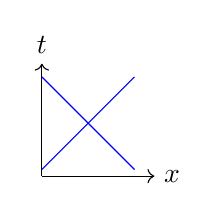
\begin{tikzpicture}[scale=0.42]
        \draw[->] (0,0) -- (3.4,0) node[right] {$x$};
        \draw[->] (0,0) -- (0,3.4) node[above] {$t$};
        \draw[blue] (0,0.2) -- (2.8,3.0);
        \draw[blue] (0,3.0) -- (2.8,0.2);
      \end{tikzpicture}\\
      {\small $x\pm at=$ 常数}
    \end{column}
    \begin{column}{0.33\textwidth}
      \centering
      抛物\\
      \begin{tikzpicture}[scale=0.42]
        \draw[->] (0,0) -- (3.4,0) node[right] {$x$};
        \draw[->] (0,0) -- (0,3.4) node[above] {$t$};
        \draw[blue] (0,0.8) -- (3.0,0.8);
        \draw[blue] (0,1.8) -- (3.0,1.8);
        \draw[blue] (0,2.8) -- (3.0,2.8);
      \end{tikzpicture}\\
      {\small 热方程：$t=$ 常数}
    \end{column}
    \begin{column}{0.32\textwidth}
      \centering
      椭圆\\
      \begin{tikzpicture}[scale=0.42]
        \draw[->] (0,0) -- (3.4,0) node[right] {$x$};
        \draw[->] (0,0) -- (0,3.4) node[above] {$y$};
        \draw[gray] (1.6,1.6) circle (1.05);
        \node at (1.6,1.6) {\small 无实特征};
      \end{tikzpicture}\\
      {\small 边界数据包围区域}
    \end{column}
  \end{columns}
\end{frame}

\begin{frame}{类型在换元下不变}
  直接计算得到
  \begin{equation*}
    A_{12}^2-A_{11}A_{22}
    =(B^2-AC)\,(\xi_x\eta_y-\xi_y\eta_x)^2.
  \end{equation*}
  雅可比的平方不为零，也不能为负，所以新判别式和 $\Delta$ 同号。
  \vspace{0.4em}

  因此双曲、抛物、椭圆是方程的性质，不是坐标系的偶然结果。标准形只是把这种性质写成最干净的主部。
\end{frame}

\subsection{三种标准形}

\begin{frame}{双曲型：沿两族特征线}
  双曲方程取两族独立的实特征线作为 $\xi$ 和 $\eta$。于是 $A_{11}=A_{22}=0$，变换后的方程变成
  \begin{equation*}
    u_{\xi\eta}
    =-\frac{1}{2A_{12}}
      \bigl(B_1u_\xi+B_2u_\eta+\widetilde C u+\widetilde F\bigr).
  \end{equation*}
  主部只剩混合导数。这是第一种标准形。
\end{frame}

\begin{frame}{双曲型：差的平方}
  再作
  \begin{equation*}
    \xi=\alpha+\beta,\qquad \eta=\alpha-\beta,
    \qquad
    \alpha=\frac{\xi+\eta}{2},\quad
    \beta=\frac{\xi-\eta}{2}.
  \end{equation*}
  链式法则给出
  \begin{align*}
    u_{\xi\eta}&=\frac14\bigl(u_{\alpha\alpha}-u_{\beta\beta}\bigr),\\
    u_\xi&=\frac12(u_\alpha+u_\beta),
    \qquad
    u_\eta=\frac12(u_\alpha-u_\beta).
  \end{align*}
\end{frame}

\begin{frame}{双曲型标准形}
  代入以后，
  \begin{equation*}
    \begin{aligned}
    u_{\alpha\alpha}-u_{\beta\beta}
    =-\frac{1}{A_{12}}\Big[&(B_1+B_2)u_\alpha
      +(B_1-B_2)u_\beta\\
      &+2\widetilde C u+2\widetilde F\Big].
    \end{aligned}
  \end{equation*}
  主部是两个纯二阶导数之差。一维波动方程已经是这个形式。
  \vspace{0.3em}

  例如 $u_{tt}-a^2u_{xx}=0$，令 $\xi=x$、$\eta=at$，则 $u_{tt}=a^2u_{\eta\eta}$，方程化为 $u_{\eta\eta}-u_{\xi\xi}=0$。
\end{frame}

\begin{frame}{抛物型：只剩一个二阶导数}
  $\Delta=B^2-AC=0$ 时，特征方程只有一个根 $\mathrm{d}y/\mathrm{d}x=B/A$。用这族特征线作 $\xi$，再选一个\textbf{不是}特征线的第二坐标 $\eta$。
  \vspace{0.3em}

  由 $\xi_x/\xi_y=-B/A$，
  \begin{align*}
    A_{11}&=\xi_y^2\left[
      A\Bigl(\frac{\xi_x}{\xi_y}\Bigr)^2
      +2B\frac{\xi_x}{\xi_y}+C\right]=0,\\
    A_{12}&=-\frac{\xi_y\eta_y}{A}(B^2-AC)=0.
  \end{align*}
  $A_{12}$ 里明确出现 $\Delta$，所以抛物型时混合项也消失。
\end{frame}

\begin{frame}{抛物型标准形}
  剩下的系数是
  \begin{equation*}
    A_{22}=\eta_y^2\left[
      \sqrt{A}\,\frac{\eta_x}{\eta_y}\pm\sqrt{C}
    \right]^2.
  \end{equation*}
  $\Delta=0$ 时主部是一个完全平方，所以只留下一个二阶方向。只要 $\eta$ 不满足特征方程，就有 $A_{22}\neq 0$。标准主部是单独一个二阶导数：
  \begin{equation*}
    u_{\eta\eta}
    =-\frac{1}{A_{22}}
      \bigl(B_1u_\xi+B_2u_\eta+\widetilde C u+\widetilde F\bigr).
  \end{equation*}
  热方程是标准的物理例子：时间导数是一阶的，空间导数是二阶的。
\end{frame}

\begin{frame}{椭圆型：复特征线}
  椭圆方程的特征坐标是共轭复数，$\eta=\xi^{*}$。写成
  \begin{equation*}
    \xi=\alpha+\mathrm{i}\beta,\qquad
    \eta=\alpha-\mathrm{i}\beta,
  \end{equation*}
  即
  \begin{equation*}
    \alpha=\frac{\xi+\eta}{2},\qquad
    \beta=\frac{\xi-\eta}{2\mathrm{i}}.
  \end{equation*}
  $\alpha,\beta$ 是实坐标。中间恒等式为
  \begin{align*}
    u_{\xi\eta}&=\frac14\bigl(u_{\alpha\alpha}+u_{\beta\beta}\bigr),\\
    u_\xi&=\frac12(u_\alpha-\mathrm{i}u_\beta),
    \qquad
    u_\eta=\frac12(u_\alpha+\mathrm{i}u_\beta).
  \end{align*}
\end{frame}

\begin{frame}{椭圆型标准形}
  混合导数形式因此变成
  \begin{equation*}
    \begin{aligned}
    u_{\alpha\alpha}+u_{\beta\beta}
    =-\frac{1}{A_{12}}\Big[&(B_1+B_2)u_\alpha
      +\mathrm{i}(B_2-B_1)u_\beta\\
      &+2\widetilde C u+2\widetilde F\Big].
    \end{aligned}
  \end{equation*}
  主部是两个纯二阶导数之和，而不是差。
  \vspace{0.3em}

  稳态温度、静电势、稳态浓度，以及无旋稳态流动，都落到这一类。
\end{frame}

\begin{frame}{分类告诉你该给什么数据}
  \begin{itemize}
    \item 一维波动方程 $u_{tt}-a^2u_{xx}=0$：双曲。要初始位移和初始速度，扰动沿特征线传播。
    \item 热方程 $u_t-\kappa u_{xx}=0$：抛物。通常给初始温度；时间的负方向上问题会不稳定。
    \item 拉普拉斯方程 $u_{xx}+u_{yy}=0$：椭圆。没有初始时刻，边界数据决定内部的场。
  \end{itemize}
  类型选错数据，问题会没有解、解不唯一，或解不连续地依赖数据。
\end{frame}

\section{本讲小结}

\begin{frame}{本讲要留下的判断}
  \begin{enumerate}
    \item 定解问题 $=$ 方程 $+$ 初始数据 $+$ 边界数据。数据写在它们各自的边界上。
    \item 三类边界条件分别指定场、法向通量，或二者的线性组合。
    \item 齐次线性问题可以叠加。稳态问题来自令时间导数为零，再用边界条件定常数。
    \item $\Delta=B^2-AC$ 的符号把二阶线性方程分成双曲、抛物、椭圆，并且在非奇异换元下不变。
  \end{enumerate}
\end{frame}

\begin{frame}{下一讲}
  第三讲把叠加原理用到两端固定的弦：
  \begin{enumerate}
    \item 分离变量，得到本征值和傅里叶正弦级数；
    \item 外力按同一组模态展开，每个模态是一个受迫振子；
    \item 圆边界上不用直角坐标，而在极坐标中分离变量，求解圆柱外的静电势。
  \end{enumerate}
\end{frame}

\end{document}
